\documentclass{article}
\usepackage{dtrt}
\usepackage{graphicx} % Required for inserting images
\usepackage{fontspec}
\usepackage{libertine}
\usepackage{enumitem}
\usepackage{fullpage}
\usepackage{amsmath}
\usepackage{tikz}
\usepackage{url}
\usepackage{hyperref}
\usetikzlibrary{arrows.meta, shapes.geometric, positioning, fit, backgrounds, calc}

% BibTeX configuration
% Format: BMS24 style (author initials + two-digit year, e.g., [BMS24])
\bibliographystyle{alpha}
\setlength{\parindent}{0pt} % No indentation for paragraphs
\setlength{\parskip}{0.5em} % Add gap between paragraphs

\title{Private Information Retrieval for Bitcoin Light Clients}
\author{Weikeng Chen}
\date{March 2026}

\begin{document}

\maketitle

\section{Introduction}

We are interested in using Private Information Retrieval (PIR) to help Bitcoin light clients synchronize with the Bitcoin network privately. A light client that knows its own keys needs to discover which unspent transaction outputs (UTXOs) it can spend, without revealing its addresses to the servers it queries. PIR enables this by allowing the client to retrieve specific database entries without the server learning which entries were accessed.

\subsection{Private Information Retrieval}

Private Information Retrieval (PIR) allows a client to retrieve an entry from a database held by one or more servers without revealing which entry is being accessed. Formally, consider a database $D$ of $N$ entries, each of $B$ bits. The client holds an index $i \in [N]$ and wishes to retrieve $D[i]$.

The trivial solution is for the client to download the entire database, achieving perfect privacy at $O(NB)$ communication cost. The goal of PIR is to achieve sublinear communication while preserving privacy.

\textbf{Single-server (computational) PIR.} A single server holds $D$. The client's query must be computationally indistinguishable from a query for any other index under some hardness assumption. The server performs computation over the query and the database to produce a response, from which the client can extract $D[i]$. The server's computation is at least $\Omega(NB)$ in the worst case (otherwise the server trivially learns that certain entries were not queried), though preprocessing and client-side hints can reduce the \emph{online} computation.

\textbf{Multi-server (information-theoretic) PIR.} The database is replicated across $t \geq 2$ non-colluding servers. Privacy holds information-theoretically: no single server (or coalition below the threshold) gains any information about $i$. The simplest 2-server scheme uses additive secret sharing of a selection vector, achieving $O(N)$ communication per server---already non-trivial compared to $O(NB)$ when $B$ is large.

\subsection{PIR Protocol Landscape}
\label{sec:landscape}

We survey practical PIR constructions across two axes: the number of servers and the amount of client-side state. We consider four settings:
\begin{itemize}[nolistsep,leftmargin=*]
    \item \textbf{Single-server:}
    \smallskip
    \begin{itemize}[nolistsep,leftmargin=*]
        \item Almost no client storage: YPIR-over-SimplePIR \cite{ypir2024}, or FHE-based schemes such as OnionPIR \cite{onionpir21} and SealPIR \cite{sealpir18}

        \item Sublinear client storage without a linear pass: SimplePIR or DoublePIR \cite{henz23}

        \item Sublinear client storage after a linear pass: Plinko \cite{plinko2024}, RMS24 \cite{rms24}, or Piano \cite{piano2024}
    \end{itemize}

    \smallskip
    \item \textbf{2-server:}
    \smallskip
    \begin{itemize}[nolistsep,leftmargin=*]
        \item Almost no client storage: DPF-PIR \cite{gilboa2014dpf,boyle2015fss,boyle2016fss}

        \item Sublinear client storage with outsourced hints: Plinko, RMS24, or Piano with hint generation delegated to a second server; or stateful PIR via pseudorandom permutations \cite{ar26fpe,checklist21}
    \end{itemize}
\end{itemize}

\subsubsection{Single-Server PIR}

We focus on single-server PIR without per-client storage on the server and allow server to preprocess the database. For protocols that do not require client storage (or if the client storage is just for some data-independent parameters), YPIR-over-SimplePIR has achieved best performance and throughput for larger blocks, in comparison to Hintless PIR \cite{li24}, Tiptoe \cite{tiptoe23}, and Spiral \cite{spiral22}.

If we allow the client to make data-dependent but sublinear storage for ``hints'', then we get better results with SimplePIR or DoublePIR, where the client downloads the hints before making any query. Note that DoublePIR is most suitable for single-bit or few-bit entries, and does not perform well when the entry size exceeds several tens of bits. This is because: (1) while the client hint is independent of the database size, it scales linearly with the entry size; and (2) this linear scaling has a very large multiplicative constant factor. This makes DoublePIR suitable for certain PIR use cases, but not the other. When using SimplePIR or DoublePIR, the server time appears to improve around $2$ times to an order of magnitudes with the sublinear hints over those that don't require hints.

If we do one step further and allow the client to download and make a linear pass over the database to generate sublinear hints (the client downloads and performs the linear pass in the streaming manner with only sublinear storage needed), then we can get much better performance with Plinko, RMS24, or Piano. The server time can be reduced by potentially two orders of magnitude. This setting works well for many devices with access to home internet or WiFi network where the network is not metered, but not all.

\subsubsection{Two-Server PIR}

We now consider PIR that assumes two servers that are non-colluding and non-communicating, meaning that the two servers do not need to know each other, and it is only the user who engages with both servers. In fact, any two trustworthy servers that have the database can be selected by the user to run this protocol. This setting is especially relevant to Bitcoin peer-to-peer (P2P) network as a user can discover two full nodes that provide this capability and use their help. The caveat is that the user needs to trust that these two servers do not collude with each other. If not, the two colluding servers can immediately learn the user's query.

The easiest way to achieve 2-server PIR is to use DPF-PIR, which is based on distributed point functions (DPF) \cite{gilboa2014dpf,boyle2015fss,boyle2016fss}. Given a share of DPF keys of size $O(logN)$, each server can expand it to $N$ bits that look random, where the two servers' bits differ exactly on the location that the user queries. Each server retrieves the entries with bit $1$ and computes an XOR sum of them. The user finally performs an XOR over the two XOR sums from the two servers and obtains the desired query result. It requires $O(NB)$ server compute time with $B$ being the entry size, but the computation is extremely lightweight. Usually, the compute can answer a PIR query close to the time that it takes to do a linear pass of the database in the storage medium (which usually is the main memory).

If we allow hint generation, as is the case in the single-server setting, we know that the server can answer the PIR queries in sublinear time, which is extremely efficient that seems to ``surpass the memory speed.'' Previously in the single-server setting, a significant downside is that the client needs to download the entire database (in a streaming manner) to generate the hint locally. Now, in the 2-server setting, the user can outsource the hint generation to one of the servers (``hint server''), and the hint can be used to query any server other than the hint server. This avoids the need for the user to download the database, and the user can directly download the hint, though it still requires sublinear client storage.

\subsubsection{Query Volume Considerations}

When we compare these different solutions, it is important to understand how many queries a user would make. For example, if a user only makes one query, then all the compute and communication costs for the hint generation may not be worthwhile if it is single-use. The overhead is not just about the client, but also the server. For single-server protocols that require a linear pass, a server needs to serve the entire database to this user. For 2-server protocols with outsourced hint generation, the hint server bears the computation cost for doing that linear pass over its local copy of the database.

This is especially relevant to Bitcoin light client synchronization because a light client may maintain a small wallet that only cares about UTXOs that the wallet can spend. In this situation, the light client knows exactly how many queries it needs to make, and after those queries, the light client has no need to access this database anymore as it has been synced up to the state that is current to the database. In this case, the client may only make one or a few queries to the database, and therefore the overhead for hint generation may not be worthwhile. An example of such a use case is when a light client imports a seed phrase or a private key, in which case it needs to identify all the UTXOs associated with the imported wallets, but this is a one-time thing.

Despite this concern, PIR is still superior than asking the light client to download the compact block filters for all the blocks since the imported key is first used (if known) and fetch a  number of blocks. First, the compact block filters for the entire Bitcoin history can still be a few gigabytes. Second, the usual way to fetch relevant blocks is to request these blocks directly from a full node by giving the block height, which leaks a little bit of privacy (which blocks this new wallet has a UTXO for). Whether this privacy leakage is acceptable depends on the situation and the user. Our goal building the PIR solution is to help those users who want to avoid this privacy leakage (which, as we will show, it is easy to avoid).

\subsubsection{Integrity and Verifiability}

Modern PIR naturally achieves privacy even against malicious servers, so we only need to focus on integrity. There are many ways to achieve integrity, some of which offer integrity against selective failure attacks \cite{kilian88,naor99,dwork99,camenisch07,lindell11,kiraz06}, while some do not. Whether it is okay to ignore selective failure attacks depends on the user and the use case. For example, a user who receives a potentially selectively failed response can continue to finish the rest of the protocol using random queries, pretending to have received a valid response, and then fetch the data from other servers.

If we ignore selective failure attacks, the most practical solution for single-server and 2-server solutions appears to be KZG polynomial commitment \cite{kzg10}, where the opening proofs are generated using the Feist-Khovratovich batch technique \cite{fk23}. An important limitation is that it uses elliptic curves, and therefore is not post-quantum. The KZG opening proof would add about 16 bytes to each entry. To reduce the PIR compute overhead caused by the additional opening proof, we can merge a few entries into one larger entry, and still only one opening proof is needed for the larger entry. With the same setup parameters of KZG, all the nodes in the network should have the same KZG polynomial commitment.

This solution, however, fails to address selective failure attacks. Selective failure attacks refer to the case when a malicious server manipulates a subset $S$ of the database entries such that if the user is reading an entry in $S$, it would fail, and if the user is reading an entry outside of $S$, it would succeed. The concern is that such a selective failure, which may be realized by the malicious server through a change of the user's subsequent actions, can leak if the user is reading an entry in $S$.

To address selective failure attacks, we can choose protocols with this additional verifiability guarantee against selective failure attacks. For single-server protocols without a linear pass, RLP26 \cite{rlp26} is a good candidate, which improves over VeriSimplePIR \cite{cl24} and significantly reduces the client hint using some one-time computation.
\begin{itemize}[nolistsep,leftmargin=*]
    \item \textbf{Single-server:}
    \smallskip
    \begin{itemize}[nolistsep,leftmargin=*]
        \item Almost no client storage: RLP26 \cite{rlp26}

        \item Sublinear client storage after a linear pass: Plinko, RMS24, or Piano with Merkle proofs, or verifiable BALANCED-PIR \cite{ar26}
    \end{itemize}

    \smallskip
    \item \textbf{2-server:} Plinko, RMS24, or Piano with Merkle proofs, or verifiable BALANCED-PIR with outsourced hint generation
\end{itemize}

Our own implementation takes a more direct route: we build SHA-256 Merkle trees over the cuckoo bins of the live database and verify retrieved bins by issuing the proof queries through the same PIR primitive the client already uses for data. This keeps the entire system post-quantum, avoids a trusted setup, and lets the same verification layer serve both the DPF and HarmonyPIR backends without protocol changes. We describe the construction in full in Section~\ref{sec:merkle}.

\subsection{Our Contributions}

We implement three distinct PIR protocols for Bitcoin UTXO lookups, each offering different trade-offs between trust assumptions, communication cost, and server computation:
\begin{itemize}[nolistsep,leftmargin=*]
    \item \textbf{DPF-PIR} (Section~\ref{sec:2server}): A 2-server stateless protocol based on Distributed Point Functions. Requires no client state and minimal communication, but assumes two non-colluding servers.
    \item \textbf{HarmonyPIR} (Section~\ref{sec:harmonypir}): A 2-server stateful protocol \cite{ar26fpe} that trades a one-time offline hint download for dramatically cheaper online queries. The hint server and query server can be different nodes.
    \item \textbf{OnionPIR} (Section~\ref{sec:onionpir}): A single-server protocol based on fully homomorphic encryption \cite{onionpir21,onionpirv2}. Eliminates the non-colluding assumption entirely at the cost of higher computation and communication.
\end{itemize}

All three protocols share the same data representation (Section~\ref{sec:data}) and batch PIR framework (Section~\ref{sec:batching}), enabling a unified system where clients can choose the protocol best suited to their threat model and network conditions.

We complement the three backends with two cross-cutting features. First, an integrity layer (Section~\ref{sec:merkle}) that builds per-group SHA-256 Merkle trees over cuckoo bins and verifies retrieved data by running the proof queries through the same PIR primitive, preserving post-quantum security and avoiding trusted setup. Second, support for \emph{delta databases} (Section~\ref{sec:delta-db}) that encode the diff between successive UTXO snapshots, letting a returning client incrementally sync by retrieving a small delta instead of re-downloading an entire snapshot.

We also provide a practical deployment (Section~\ref{sec:deployment}) including browser-based clients via WebAssembly \cite{wasm} and an Electrum wallet plugin \cite{electrum} with all three backends, a multi-database server architecture, and a client-side sync planner that chooses between full and delta databases.

\subsection{Paper Organization}

Section~\ref{sec:data} describes the Bitcoin UTXO model, our data representation, and techniques for reducing the UTXO set size. Section~\ref{sec:batching} presents the PIR-variant-agnostic batch PIR framework using Probabilistic Batch Codes. Sections~\ref{sec:2server},~\ref{sec:harmonypir}, and~\ref{sec:onionpir} detail the three protocol instantiations: DPF-PIR, HarmonyPIR, and OnionPIR, respectively. Section~\ref{sec:merkle} describes the per-group Merkle integrity layer, and Section~\ref{sec:delta-db} describes delta databases and incremental sync. Section~\ref{sec:comparison} compares the three protocols across multiple dimensions. Section~\ref{sec:deployment} describes the implementation and deployment, including the multi-database catalog, browser and wallet integration.


\clearpage

\section{Data Representation}
\label{sec:data}

\subsection{Bitcoin UTXO Model}

Bitcoin uses an Unspent Transaction Output (UTXO) model. Each transaction consumes previous outputs (inputs) and creates new outputs. The set of all outputs that have not yet been spent forms the \emph{UTXO set}, which represents the current state of all spendable coins.

Each UTXO is uniquely identified by a pair (TXID, vout), where TXID is the 32-byte hash of the creating transaction and vout is the output index within that transaction. Each UTXO carries an \emph{amount} (in satoshis) and a \emph{ScriptPubKey}---a locking script that specifies the conditions under which the output can be spent.

Common ScriptPubKey types include:
\begin{itemize}[nolistsep,leftmargin=*]
    \item \textbf{P2PKH} (Pay-to-Public-Key-Hash): Legacy addresses starting with \texttt{1}
    \item \textbf{P2SH} (Pay-to-Script-Hash): Script hash addresses starting with \texttt{3}
    \item \textbf{P2WPKH / P2WSH} (Pay-to-Witness-*): SegWit addresses starting with \texttt{bc1q}
    \item \textbf{P2TR} (Pay-to-Taproot): Taproot addresses starting with \texttt{bc1p}
\end{itemize}

A \emph{light client} knows its own private keys (and thus its addresses and ScriptPubKeys) but does not maintain a full copy of the blockchain. To spend its coins, the light client needs to discover which UTXOs are locked to its ScriptPubKeys and retrieve the corresponding (TXID, vout, amount) tuples. PIR enables this discovery without revealing the client's addresses to the server.

\subsection{Data Organization}

\textbf{Sort and group.} The server sorts UTXOs by ScriptPubKey hash, then packs them into fixed-size chunks. Each chunk stores complete UTXO records including full 32-byte TXIDs, vout indices, and amounts. Multiple ScriptPubKeys may share a chunk via bin-packing.

\textbf{Index map.} Maps each ScriptPubKey (via its RIPEMD-160 hash) to the chunk location and data length. This is organized as a cuckoo hash table for $O(1)$ keyword-to-index lookup \cite{PR01}. Each index slot is 13 bytes: an 8-byte fingerprint tag (derived from the script hash, used to select the correct slot within a retrieved bin), a 4-byte starting chunk identifier, and a 1-byte chunk count.

\textbf{Chunk map.} Stores the actual UTXO data in fixed-size 40-byte blocks. Full 32-byte TXIDs are stored directly in the chunks, eliminating a separate TXID resolution step. Each chunk slot is 44 bytes: a 4-byte chunk identifier followed by 40 bytes of UTXO data. The chunk map is also organized as a cuckoo hash table for PIR-compatible retrieval.

\subsection{Cuckoo Hashing for Keyword Lookup}

Cuckoo hashing \cite{PR01} is a hashing scheme that provides worst-case $O(1)$ lookup time. To store $n$ items, we maintain a table of $T$ bins, each holding $s$ slots, with $h$ independent hash functions $H_1, \ldots, H_h$.

Each item $x$ can reside in any of its $h$ candidate bins $H_1(x), \ldots, H_h(x)$. To insert $x$: if any candidate bin has a free slot, place $x$ there. Otherwise, evict a random existing item from one candidate bin, insert $x$, and re-insert the evicted item recursively. With appropriate choices of $h$ and $s$ (e.g., $h{=}2, s{=}3$ or $h{=}3, s{=}2$), load factors above 95\% are achievable.

\textbf{PIR by keyword.} Cuckoo hashing enables PIR by keyword (as opposed to PIR by index). Given a keyword $w$, the client computes its $h$ candidate bin indices and issues PIR queries for those bins. Upon retrieving the bin contents, the client checks which slot (if any) contains an entry matching $w$. This transforms the problem of searching an unordered key-value store into a constant number of PIR-by-index queries.

We use two distinct terms throughout the rest of the paper to avoid collisions. A \emph{bin} is a location in one of these keyword-lookup cuckoo tables: a row of $s$ slots that a PIR query retrieves atomically. A \emph{group} refers to the outer sharding used by batch PIR (Section~\ref{sec:batching}): the database is partitioned into $K$ groups, one cuckoo table per group, and a batch of client queries is distributed across the $K$ groups so that each group answers at most one real query per round.

\subsection{Reducing the UTXO Set}
\label{sec:extension}

Since the PIR service is designed for light clients who do not frequently run the Bitcoin node for synchronization or for newly imported wallet addresses from a regular user, we can realistically expect that the user only makes a few transactions, keeps only a few UTXOs in the chain, and has no intention to create large number of dust outputs (a typical pattern of some Bitcoin layer-2 protocols). Therefore, taking this in mind, we can reduce the UTXO set by filtering out scriptPubKeys that show different user patterns, or, if not filtering out the entire scriptPubKey, we can selectively filter out certain transactions or certain UTXOs that match some profiles.

For example, a scriptPubKey that has been involved in a significantly above average number of UTXOs is likely not a regular user and probably should run its own full node to have the full security and privacy.

Another example is that we can filter out UTXOs that are of dust amount. It is possible that a honest user has dust UTXOs and may want to use them in the future, but given that each dust UTXO is worth probably like $0.4$ USD, we can say that they are of a lower prioirity, and a user who sincerely wants to use them should first try to avoid generating dust UTXOs as it should not occur naturally, and if the user sincerely wants to recover from the dust amount, the user is recommended to use an RPC server (maybe through Tor), or if strict privacy is a concern, run a full node---honestly speaking, if the user wants to consolidate these dust UTXOs, the other full nodes are going to learn it sooner or later anyway because they can wait for the consolidation transaction.

If we worry that the dust amount filtering might be excessive, we can also target certain protocols that are known to generate a large number of dust UTXOs, such as the Omnilayer, by looking into the \textrm{OP\_RETURN} output next to the dust UTXO and checking if it starts with ``omni''.

We can also make a list of known exchange wallet addresses and filter them out given that these crypto exchange is definitely not running a light client. There are some services for this purpose, such as Arkham, that provides a list of identified addresses of notable market paricipants (who are unlikely using this light client).


\clearpage

\section{Batch PIR}
\label{sec:batching}

A light client typically needs to look up multiple ScriptPubKeys simultaneously. This section describes how we use Probabilistic Batch Codes (PBC) to amortize the cost of multiple PIR queries, and how the two-level architecture (index map then chunk map) composes with batching. The batch PIR framework described here is PIR-variant-agnostic: it works with any underlying single-query PIR scheme, including the 2-server DPF-PIR instantiation in Section~\ref{sec:2server}.

\subsection{Batch PIR and Probabilistic Batch Codes}

\textbf{Batch PIR} \cite{IKOS04} addresses the problem of retrieving $m$ entries simultaneously. The naive approach---issuing $m$ independent PIR queries---costs $m$ times the single-query cost. Batch PIR aims to reduce this by amortizing work across queries.

\textbf{Probabilistic Batch Codes (PBC)} achieve batch PIR by distributing $m$ queries across $K$ \emph{groups} (with $K > m$) such that each group contains at most one real query. The construction uses cuckoo hashing:
\begin{enumerate}[nolistsep,leftmargin=*]
    \item For each of the $m$ queries, compute $h$ candidate groups using cuckoo hash functions.
    \item Place queries into groups via cuckoo insertion with eviction chains.
    \item Pad all empty groups with random dummy queries.
    \item Issue $K$ independent PIR queries in parallel---one per group.
\end{enumerate}

Since each group holds at most one real query, the server processes $K$ single-entry PIR queries. For DPF-PIR, this means generating $K$ DPF key pairs and having each server perform $K$ XOR-sum computations. The effective cost per query drops from $O(NB)$ to $O(NB \cdot K/m)$ when the server can share work across the $K$ evaluations.

Each of the $K$ groups is itself a cuckoo hash table in the sense of Section~\ref{sec:data}, where the inner rows are called \emph{bins}. We consistently use ``group'' for the outer PBC sharding and ``bin'' for the inner cuckoo row; this matches the terminology used throughout our codebase.

\subsection{Two-Level Query Architecture}

Our system uses a two-level architecture: an \emph{index map} that locates data, and a \emph{chunk map} that stores the actual UTXO data (see Section~\ref{sec:data} for the data layout). A complete UTXO lookup requires two rounds of batch PIR:

\begin{figure}[htbp]
\centering
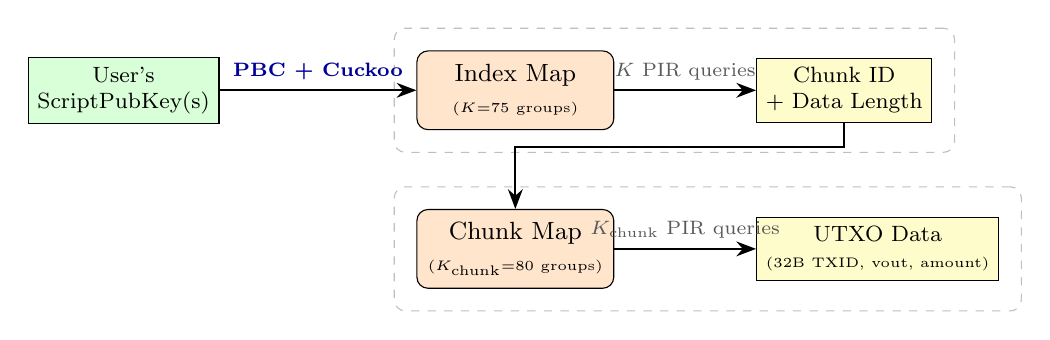
\begin{tikzpicture}[
    node distance=1.2cm and 1.8cm,
    box/.style={rectangle, draw, rounded corners, minimum width=2.5cm, minimum height=1cm, align=center, font=\small},
    data/.style={rectangle, draw, fill=blue!10, minimum width=1.8cm, minimum height=0.7cm, align=center, font=\footnotesize},
    arrow/.style={-{Stealth[length=2.5mm]}, thick},
    label/.style={font=\scriptsize, text=gray!70!black},
    pirlabel/.style={font=\scriptsize\bfseries, text=blue!60!black}
]

\node[data, fill=green!15] (user) {User's\\ScriptPubKey(s)};
\node[box, fill=orange!20, right=2.5cm of user] (map1) {Index Map\\{\tiny ($K{=}75$ groups)}};
\node[data, fill=yellow!20, right=of map1] (chunkinfo) {Chunk ID\\+ Data Length};
\node[box, fill=orange!20, below=1cm of map1] (map2) {Chunk Map\\{\tiny ($K_\text{chunk}{=}80$ groups)}};
\node[data, fill=yellow!20, right=of map2] (utxo) {UTXO Data\\{\tiny (32B TXID, vout, amount)}};

\draw[arrow] (user) -- (map1) node[midway, above, pirlabel] {PBC + Cuckoo};
\draw[arrow] (map1) -- (chunkinfo) node[midway, above, label] {$K$ PIR queries};
\draw[arrow] (chunkinfo.south) -- ++(0,-0.3) -| (map2.north);
\draw[arrow] (map2) -- (utxo) node[midway, above, label] {$K_\text{chunk}$ PIR queries};

\begin{scope}[on background layer]
    \node[fit=(map1)(chunkinfo), draw=gray!50, dashed, rounded corners, inner sep=8pt, label={[font=\tiny\itshape, text=gray]above:Level 1}] {};
    \node[fit=(map2)(utxo), draw=gray!50, dashed, rounded corners, inner sep=8pt, label={[font=\tiny\itshape, text=gray]left:Level 2}] {};
\end{scope}

\end{tikzpicture}
\caption{Two-level batch PIR architecture. The client issues $K$ parallel PIR queries per level, using Probabilistic Batch Codes to pack multiple lookups into a single round.}
\label{fig:two-maps}
\end{figure}

\textbf{Level 1: Index lookup.} The client computes RIPEMD-160 hashes of all queried ScriptPubKeys, derives $h$ candidate groups per query via cuckoo hash functions, and places them into $K$ PBC groups. For each group, the client generates a PIR query targeting the assigned bin in the group's index cuckoo table and sends it to the server(s). The responses are combined to recover index slots containing starting chunk ids and chunk counts.

\textbf{Level 2: Chunk retrieval.} Using the chunk locations from Level~1, the client repeats the process with $K_\text{chunk}$ PBC groups over the chunk database. The recovered chunks contain full UTXO records: 32-byte TXIDs, vout indices, and amounts in satoshis---everything needed to construct a spending transaction. Each chunk is 40 bytes; each slot in the chunk cuckoo table is 44 bytes (4-byte chunk identifier plus 40-byte payload).

\textbf{Distributional PIR.} We can apply distributional PIR \cite{lehmkuhl25} to optimize for the common case: most light clients hold few UTXOs under common script types, while whale addresses with thousands of UTXOs likely run full nodes. By tuning the PIR parameters for the more likely queries, the average server cost decreases without eliminating the ability to query less common entries.

\begin{table}[htbp]
\centering
\begin{tabular}{|l|c|c|c|c|c|}
\hline
\textbf{Database} & \textbf{Slot Size} & \textbf{Groups ($K$)} & \textbf{Cuckoo} & \textbf{DPF queries/group} & \textbf{PIR domain} \\
\hline
Index (Level 1) & 13 B & 75 & 2-hash, 4 slots/bin & 2 & $2^{20}$ \\
Chunks (Level 2) & 44 B & 80 & 2-hash, 3 slots/bin & 2 & $2^{21}$ \\
\hline
\end{tabular}
\caption{Batch PIR parameters. Each level uses $K$ parallel PIR queries over cuckoo hash tables, one table per group. Each DPF query retrieves one cuckoo bin: 4 slots $\times$ 13 B = 52 B for the index level, and 3 slots $\times$ 44 B = 132 B for the chunk level.}
\label{tab:databases}
\end{table}


\clearpage

\section{2-Server Stateless PIR via DPF}
\label{sec:2server}

This section describes the 2-server stateless PIR instantiation of our system, based on Distributed Point Functions (DPF). The client requires no persistent state or hints---only the DPF keys generated fresh for each query session. Combined with the batch PIR framework from Section~\ref{sec:batching}, this yields a complete system for private UTXO lookups.

\subsection{Distributed Point Functions (DPF)}
\label{sec:dpf}

A Distributed Point Function (DPF) \cite{gilboa2014dpf,boyle2015fss,boyle2016fss} is a cryptographic primitive that enables efficient 2-server PIR. A \emph{point function} $f_{\alpha,\beta}$ evaluates to $\beta$ at input $\alpha$ and to $0$ everywhere else. A DPF splits this point function into two keys $(k_0, k_1)$ such that:
\begin{itemize}[nolistsep,leftmargin=*]
    \item \textbf{Correctness:} $\text{Eval}(k_0, x) \oplus \text{Eval}(k_1, x) = f_{\alpha,\beta}(x)$ for all $x$.
    \item \textbf{Security:} Each individual key $k_b$ is computationally indistinguishable from a key for any other point function.
\end{itemize}

Each key has size $O(\lambda \log N)$ where $\lambda$ is the security parameter and $N$ is the domain size. To perform PIR on a database of $N$ entries indexed by $[N]$:
\begin{enumerate}[nolistsep,leftmargin=*]
    \item The client generates DPF keys $(k_0, k_1)$ for the point function $f_{i, 1}$ where $i$ is the target index.
    \item Server $b$ expands $k_b$ to obtain a vector of $N$ field elements and computes $r_b = \bigoplus_{x=0}^{N-1} \text{Eval}(k_b, x) \cdot D[x]$.
    \item The client recovers $D[i] = r_0 \oplus r_1$.
\end{enumerate}

The server computation is $O(NB)$ but consists of simple XOR operations over the database, making it extremely fast in practice---often close to the speed of a single linear pass over the data in memory.

\subsection{Implementation}
\label{sec:implementation}

We have implemented a complete system based on the 2-server DPF-PIR approach with Probabilistic Batch Codes (PBC), as described in Section~\ref{sec:batching}. The implementation consists of database generation tools (Rust), two PIR servers (Rust with \texttt{tokio}), and client libraries (Rust CLI and TypeScript/Web). The two-level architecture from Figure~\ref{fig:two-maps} eliminates the TXID resolution step of earlier designs by storing full 32-byte TXIDs directly in the UTXO chunks.

\subsubsection{System Architecture}

Each server maintains identical copies of the index and chunk databases, loaded via memory-mapped files (\texttt{memmap2}). The client connects to both servers over WebSocket and distributes DPF key shares, so neither server learns the query target unless they collude. Communication uses a compact binary protocol supporting database discovery, batch PIR queries, and connection health checks.

\begin{figure}[htbp]
\centering
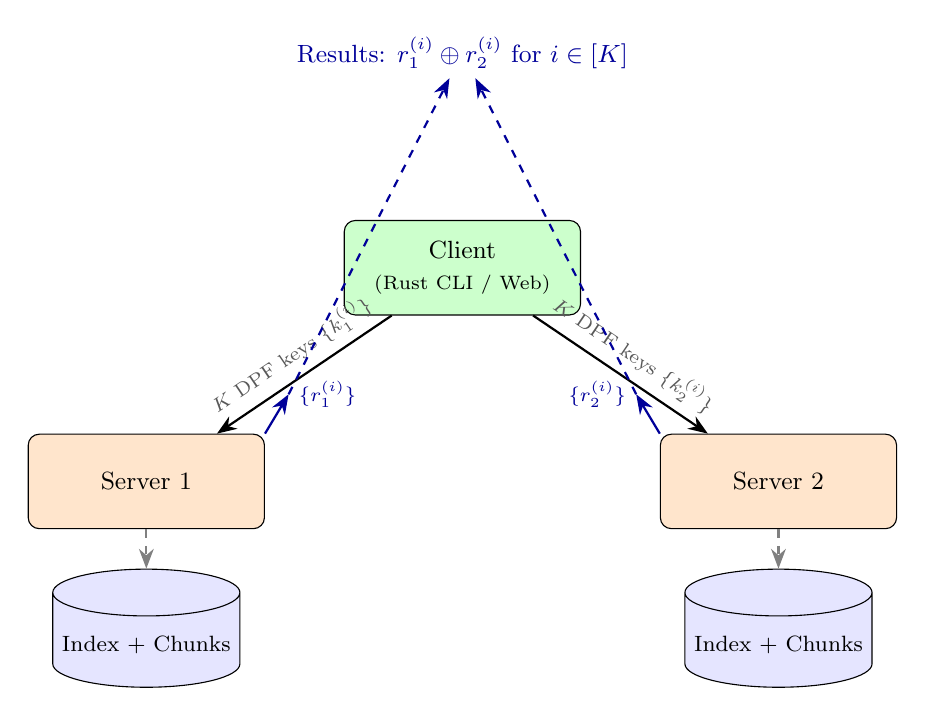
\begin{tikzpicture}[
    node distance=1.5cm and 2cm,
    box/.style={rectangle, draw, rounded corners, minimum width=3cm, minimum height=1.2cm, align=center, font=\small},
    db/.style={cylinder, draw, shape border rotate=90, aspect=0.25, minimum height=1.5cm, minimum width=1.2cm, fill=blue!10, font=\footnotesize},
    arrow/.style={-{Stealth[length=2.5mm]}, thick},
    label/.style={font=\scriptsize, text=gray!70!black}
]

\node[box, fill=green!20] (client) {Client\\{\scriptsize (Rust CLI / Web)}};
\node[box, fill=orange!20, below left=1.5cm and 1cm of client] (server1) {Server 1};
\node[box, fill=orange!20, below right=1.5cm and 1cm of client] (server2) {Server 2};
\node[db, below=0.5cm of server1] (db1) {Index + Chunks};
\node[db, below=0.5cm of server2] (db2) {Index + Chunks};

\draw[arrow] (client) -- (server1) node[midway, above, sloped, label] {$K$ DPF keys $\{k_1^{(i)}\}$};
\draw[arrow] (client) -- (server2) node[midway, above, sloped, label] {$K$ DPF keys $\{k_2^{(i)}\}$};
\draw[arrow, dashed, gray] (server1) -- (db1);
\draw[arrow, dashed, gray] (server2) -- (db2);

\draw[arrow, blue!60!black] (server1.north east) -- ++(0.3, 0.5) node[right, font=\scriptsize] {$\{r_1^{(i)}\}$};
\draw[arrow, blue!60!black] (server2.north west) -- ++(-0.3, 0.5) node[left, font=\scriptsize] {$\{r_2^{(i)}\}$};

\node[above=1.8cm of client, font=\small, text=blue!60!black] (xor) {Results: $r_1^{(i)} \oplus r_2^{(i)}$ for $i \in [K]$};
\draw[arrow, blue!60!black, dashed] ($(server1.north east)+(0.3, 0.5)$) -- (xor);
\draw[arrow, blue!60!black, dashed] ($(server2.north west)+(-0.3, 0.5)$) -- (xor);

\end{tikzpicture}
\caption{Two-server batch DPF-PIR architecture. The client generates $K$ DPF key pairs (one per PBC group) and sends the shares to each server. Each server computes $K$ XOR sums in parallel; the client combines responses to recover all queried entries.}
\label{fig:architecture}
\end{figure}

\subsubsection{Database Generation}

The offline pipeline transforms raw Bitcoin blockchain data into two PIR-queryable databases. Each stage is a separate Rust binary in the \texttt{build} crate.

\textbf{Pipeline overview:}
\begin{enumerate}[nolistsep,leftmargin=*]
    \item \textbf{UTXO extraction:} Parse the UTXO snapshot (\texttt{dumptxoutset}) to extract ScriptPubKey hashes, full 32-byte TXIDs, vout indices, and amounts.
    \item \textbf{Chunk generation:} Group UTXOs by ScriptPubKey, serialize with VarInt encoding, and pack into fixed-size 40-byte blocks. Each block stores complete records including full TXIDs.
    \item \textbf{Index construction:} Build an index mapping each ScriptPubKey hash to its chunk location and count. Each index slot is 13 bytes: an 8-byte fingerprint tag (derived from the script hash) + 4-byte starting chunk id + 1-byte chunk count.
    \item \textbf{Cuckoo hashing:} Organize both databases into cuckoo hash tables for PBC-compatible batch retrieval. Both use 2 cuckoo hash functions; the index database has 4 slots per bin and the chunk database has 3 slots per bin, both achieving $>$95\% load factor with zero stash.
    \item \textbf{(Optional) Per-group Merkle:} Build per-group SHA-256 Merkle trees over the cuckoo bins, emit flat sibling tables (one file per level), a tree-top cache, and a super-root, enabling integrity verification through the same DPF primitive (Section~\ref{sec:merkle}).
    \item \textbf{Verification:} Validate that all entries are retrievable from the cuckoo tables.
\end{enumerate}

\textbf{Dual role of cuckoo hashing.} Cuckoo hashing serves two purposes in our system. First, it provides PIR-by-keyword: given a ScriptPubKey, the client computes candidate bin indices to locate data without scanning. Second, it implements PBC for batch PIR: when querying $m$ entries, each query maps to $3$ candidate groups; the client places queries into $K$ total groups via cuckoo insertion, and all $K$ DPF queries execute in parallel. The index level uses 2 cuckoo hash functions with $4$ slots per bin, and the chunk level uses 2 cuckoo hash functions with $3$ slots per bin. Each DPF query returns one cuckoo bin: $4 \times 13 = 52$ bytes for the index level, and $3 \times 44 = 132$ bytes for the chunk level.

\subsubsection{Query Protocol}

A complete UTXO lookup requires two rounds of batch PIR:

\textbf{Level 1: Index lookup.} The client computes RIPEMD-160 hashes of all queried ScriptPubKeys, derives 3 candidate groups per query via cuckoo hash functions (\texttt{splitmix64}-based), and places them into $K{=}75$ PBC groups. For each group, the client generates 2 DPF key pairs (one per cuckoo hash function in the 2-hash index cuckoo) and sends one share of each to each server. The servers expand all DPF keys and return XOR sums. The client combines responses to recover 13-byte index slots containing fingerprint tags, starting chunk ids, and chunk counts. The client matches the recovered tag against the expected tag for its ScriptPubKey to identify the correct slot within the 4-slot cuckoo bin.

\textbf{Level 2: Chunk retrieval.} Using the chunk locations from Level~1, the client repeats the process with $K_\text{chunk}{=}80$ PBC groups over the chunk database. The chunk cuckoo uses 2 hash functions with 3 slots per bin, so the client generates 2 DPF key pairs per group. The recovered 132-byte results (3 slots $\times$ 44 bytes each) contain chunk identifiers and full UTXO records: 32-byte TXIDs, vout indices, and amounts in satoshis---everything needed to construct a spending transaction.

\subsubsection{Client Implementations}

\textbf{Rust CLI.} Command-line tool that takes ScriptPubKeys as hex, performs the two-level batch PIR protocol, and outputs decoded UTXO data.

\textbf{Web client (TypeScript).} Browser-compatible library using WebSocket connections. Implements DPF key generation, cuckoo hashing, and PBC placement in pure TypeScript. Supports Bitcoin address input (P2PKH, P2SH, P2WPKH, P2WSH, P2TR) with automatic conversion to ScriptPubKey.

\textbf{Electrum plugin (Python).} Integration with the Electrum Bitcoin wallet \cite{electrum} that replaces its native synchronizer with PIR-based UTXO discovery. See Section~\ref{sec:deployment} for details on all client implementations.


\clearpage

\section{2-Server Stateful PIR via HarmonyPIR}
\label{sec:harmonypir}

This section describes the 2-server \emph{stateful} PIR instantiation based on HarmonyPIR \cite{ar26fpe}, which uses pseudorandom permutations (PRPs) to organize hints that enable sublinear online queries. Unlike DPF-PIR, HarmonyPIR requires a one-time offline phase where the client downloads precomputed hints, but in return achieves dramatically lower per-query communication and server computation.

\subsection{Overview}

HarmonyPIR is a stateful PIR protocol in the offline/online model, following the line of work initiated by Checklist \cite{checklist21}. The system involves two servers with distinct roles:
\begin{itemize}[nolistsep,leftmargin=*]
    \item \textbf{Hint server} (offline): Computes and streams PRP-based hint parities to the client. This is a one-time operation per session.
    \item \textbf{Query server} (online): Answers indexed lookups by returning the XOR of requested database entries. Each query requires only $O(\sqrt{N})$ server work.
\end{itemize}

The key trade-off is: HarmonyPIR incurs a large offline download (hundreds of megabytes of hints) but achieves per-query online communication and server computation that is \emph{sublinear} in the database size. This makes it well-suited for clients that will issue many queries---such as a light client synchronizing multiple wallet addresses.

The client maintains a limited \emph{query budget} of approximately $M = N/T$ queries per hint set, where $N$ is the database size and $T = \lfloor\sqrt{2N}\rceil$. Once the budget is exhausted, the client must re-download hints.

\subsection{Offline Phase: Hint Generation}
\label{sec:harmony-offline}

In the offline phase, the hint server computes a compact representation of the database that allows the client to later recover individual entries using only $O(\sqrt{N})$ work per query.

\textbf{Setup.} Let $\mathsf{DB}[0], \ldots, \mathsf{DB}[N{-}1]$ denote the database entries, each of $w$ bytes. Let $P: [N'] \to [N']$ be a pseudorandom permutation over a padded domain of size $N' \geq N$ (chosen so that $2N' \bmod T = 0$). Define the parameters:
\begin{align*}
    T &= \lfloor\sqrt{2N}\rceil, \\
    M &= N'/T \quad \text{(number of segments)}.
\end{align*}

\textbf{Hint computation.} The server computes $M$ hint values, each of $w$ bytes, via a scatter-XOR operation:
$$H[s] = \bigoplus_{\substack{k \in [N] \\ \lfloor P(k)/T \rfloor = s}} \mathsf{DB}[k], \quad s \in [M].$$
That is, each database row $k$ is assigned to segment $s = \lfloor P(k)/T \rfloor$ by the PRP, and the hint for segment $s$ is the XOR of all rows assigned to it. Rows in the range $[N, N')$ are virtual zero-rows and do not affect the XOR. The total hint size is $M \times w$ bytes per group.

\textbf{Per-group hints.} The system maintains 155 independent HarmonyPIR instances---one per PBC group (75 index-level + 80 chunk-level). Each instance uses a distinct PRP key derived from a shared master key by XORing the group identifier into bytes 12--15 of the key. The hint server computes and streams hints for all 155 groups, using batch parallelism for efficiency.

\subsection{Online Phase: Querying}
\label{sec:harmony-online}

To query for a database entry at index $q$, the client proceeds as follows:

\begin{enumerate}[nolistsep,leftmargin=*]
    \item \textbf{Locate via PRP:} Compute the cell $c = P(q)$. Determine the segment $s = \lfloor c/T \rfloor$ and position $r = c \bmod T$.

    \item \textbf{Build request:} Construct the set of indices to request from the query server---namely, all database rows that the PRP maps into segment $s$, \emph{except} for the target row $q$ itself. Formally, the request set is:
    $$R = \{P^{-1}(s \cdot T + j) : j \in [T], j \neq r\} \cap [N].$$
    The client sends $R$ (as sorted $\mathsf{u32}$ indices) to the query server.

    \item \textbf{Server response:} The query server returns the XOR of the requested entries: $\bigoplus_{i \in R} \mathsf{DB}[i]$.

    \item \textbf{Recover answer:} The client XORs the server's response with the stored hint $H[s]$:
    $$\mathsf{DB}[q] = H[s] \oplus \bigoplus_{i \in R} \mathsf{DB}[i].$$
    This works because $H[s]$ is the XOR of \emph{all} rows in segment $s$ (including $\mathsf{DB}[q]$), and the server returned the XOR of all rows \emph{except} $\mathsf{DB}[q]$.

    \item \textbf{State update (relocation):} After recovering $\mathsf{DB}[q]$, the client updates its local data structure so that future queries remain correct. This involves ``relocating'' row $q$ within the hint structure so that the same segment is not queried twice for the same position.
\end{enumerate}

Each online query involves sending $O(T) = O(\sqrt{N})$ indices and receiving $w$ bytes back. The query server's work is also $O(T \cdot w)$---a linear scan over roughly $\sqrt{N}$ entries---which is sublinear in the database size $N$.

\subsection{Dummy Queries}
\label{sec:harmony-dummies}

To prevent the server from distinguishing real queries from padding, the client generates \emph{synthetic dummy} queries for PBC groups that do not hold a real query in a given round.

A synthetic dummy is constructed by sampling a count $c \sim \text{Binomial}(T, 0.5)$ and then choosing $c$ indices uniformly at random from $[N]$. The resulting request has the same format as a real query but does not modify the client's hint state. This ensures that the distribution of request sizes and content is statistically indistinguishable from real queries to the server.

\subsection{Integration with Batch PIR}
\label{sec:harmony-batch}

HarmonyPIR plugs into the same PBC framework described in Section~\ref{sec:batching}. The client maintains 155 independent HarmonyPIR group instances:
\begin{itemize}[nolistsep,leftmargin=*]
    \item \textbf{Index level:} $K{=}75$ groups, each with entry size $w = 52$ bytes (one cuckoo bin = 4 slots $\times$ 13 bytes per index slot).
    \item \textbf{Chunk level:} $K_\text{chunk}{=}80$ groups, each with entry size $w = 132$ bytes (one cuckoo bin = 3 slots $\times$ 44 bytes per chunk slot).
\end{itemize}

The query protocol proceeds in rounds, analogous to DPF-PIR:
\begin{enumerate}[nolistsep,leftmargin=*]
    \item The client places $m$ ScriptPubKey queries into $K$ PBC groups via cuckoo hashing (same as Section~\ref{sec:batching}).
    \item For each of the 2 cuckoo hash function rounds at the index level:
    \begin{itemize}[nolistsep,leftmargin=*]
        \item Groups with a real query generate a HarmonyPIR request targeting the assigned cuckoo bin.
        \item Groups without a real query generate a synthetic dummy.
    \end{itemize}
    \item All $K$ requests are sent to the query server in a single batch. The server responds with $K$ XOR results.
    \item The client processes responses: real queries recover index slots via the hint XOR; dummy responses are discarded.
    \item The process repeats for the chunk level with $K_\text{chunk}$ groups.
\end{enumerate}

\subsection{PRP Backend Selection}
\label{sec:prp-backends}

The PRP $P$ must be a permutation over a domain of size $N'$ (typically $\sim 10^6$), which is far smaller than the $2^{128}$ domain of standard block ciphers like AES. Several small-domain PRP constructions are available, each with different performance characteristics:

\begin{itemize}[nolistsep,leftmargin=*]
    \item \textbf{Hoang (swap-or-not) \cite{hoang12}:} A Feistel-like construction based on card shuffles. Uses AES round functions with 4-way pipelining. This is the default backend and serves as the baseline.

    \item \textbf{FastPRP:} A radix-sort-based PRP with $O(N \log N)$ batch evaluation. Precomputes the entire permutation table, trading memory for speed. Achieves $2$--$4\times$ speedup over Hoang.

    \item \textbf{ALF \cite{alf25}:} An AES-NI-based format-preserving encryption scheme optimized for SIMD execution. Achieves the best performance: $4$--$8\times$ faster than Hoang. Requires hardware AES-NI support (available on modern x86 and ARM processors, and via WASM SIMD128 in browsers).
\end{itemize}

The PRP backend is selected at session initialization and must be consistent between the hint server and client. Server-side benchmarks on a 24-thread machine show ALF computing all 75 index hints in $\sim$711~ms, compared to $\sim$1.05~s for FastPRP and $\sim$7.24~s for Hoang.

\subsection{Hint Caching and Query Budget}
\label{sec:harmony-caching}

Each HarmonyPIR group instance supports approximately $M \approx N/T \approx \sqrt{N/2}$ queries before its hints are exhausted, where $N$ here refers to the number of cuckoo bins in the group's table. For the current main database this gives roughly $530$ queries per group at the INDEX level (where $N \approx 565{,}000$ bins, DPF domain $2^{20}$) and roughly $730$ queries per group at the CHUNK level (where $N \approx 1{,}064{,}000$ bins, DPF domain $2^{21}$). Both levels comfortably exceed typical wallet query volumes.

To avoid re-downloading hints unnecessarily, the client caches hint state:
\begin{itemize}[nolistsep,leftmargin=*]
    \item \textbf{State serialization:} Each group's full state (hints, PRP key, relocation structure, query counter) can be serialized and stored in the browser's \texttt{localStorage} or on disk.
    \item \textbf{Exhaustion detection:} Before each batch query, the client checks the minimum remaining query budget across all active groups. If any group is exhausted, the client triggers a hint refresh from the hint server.
    \item \textbf{Resilient reconnection:} If the WebSocket connection drops mid-session, the client reconnects with exponential backoff and resumes using cached state, avoiding a full hint re-download.
\end{itemize}


\clearpage

\section{1-Server PIR via OnionPIR}
\label{sec:onionpir}

This section describes the single-server PIR instantiation based on OnionPIR \cite{onionpir21} and its successor OnionPIRv2 \cite{onionpirv2}, a fully homomorphic encryption (FHE) based protocol. Unlike DPF-PIR and HarmonyPIR, OnionPIR requires only \emph{one} server and provides computational privacy under lattice hardness assumptions, eliminating the need for a non-colluding server pair. The trade-off is higher communication cost and server computation per query.

\subsection{Overview}

OnionPIR uses the composition of two somewhat homomorphic encryption (SHE) schemes---BFV-style encryption and GSW-style encryption---to achieve compact responses. The client encrypts its query index under an FHE scheme, the server homomorphically evaluates a selection function over the encrypted query and the database, and the client decrypts the result to obtain the desired entry.

The protocol is \emph{stateless}: the client generates fresh encryption keys per session and requires no hints or prior database knowledge. The FHE parameters used in our instantiation are:
\begin{itemize}[nolistsep,leftmargin=*]
    \item Polynomial degree: $d = 2048$
    \item Plaintext modulus: $p = 32{,}771$ (a 15-bit prime)
    \item Entry size: $d \times 15 / 8 = 3840$ bytes (fixed by the FHE parameters)
\end{itemize}

The fixed 3840-byte entry size is a fundamental constraint of OnionPIR's encoding: each database entry occupies exactly one RLWE plaintext polynomial, with 15 usable bits per coefficient across 2048 coefficients.

\subsection{Database Layout}
\label{sec:onion-layout}

Because OnionPIR's entry size (3840 bytes) is much larger than the DPF/HarmonyPIR entry sizes (39 or 132 bytes), we use a different database layout that packs multiple logical records into each 3840-byte OnionPIR entry.

\subsubsection{Index Level (75 Groups)}

Each PBC group's index database is organized as a cuckoo hash table where each bin is packed with up to 256 index slots, fitting exactly into one 3840-byte entry:
\begin{itemize}[nolistsep,leftmargin=*]
    \item \textbf{Slot format:} 15 bytes per slot---8-byte fingerprint tag, 4-byte entry identifier (pointing into the main database), 2-byte byte offset within the entry, and 1-byte entry count.
    \item \textbf{Bin packing:} $256 \times 15 = 3840$ bytes per bin, matching one OnionPIR entry.
    \item \textbf{Cuckoo design:} 2 hash functions over $\sim$8,840 bins per group.
\end{itemize}

The client computes both candidate bin indices, issues one OnionPIR query per candidate, and scans the returned 256 slots for a matching fingerprint tag.

\subsubsection{Main Database (80 Groups)}

UTXO data is greedily packed into 3840-byte entries:
\begin{itemize}[nolistsep,leftmargin=*]
    \item Multiple addresses share a single entry via greedy bin-packing. If an address's serialized UTXO data does not fit in the remaining space of the current entry, padding is inserted and a new entry begins.
    \item From approximately 53.6 million addresses, the packing produces $\sim$815,000 unique entries with $\sim$95.9\% packing efficiency.
    \item Each entry is assigned to 3 of the 80 PBC groups (triplication for batch PIR).
    \item Within each group, entries are placed into a cuckoo hash table with 6 hash functions, 1 slot per bin, and $\sim$32,000 bins per group.
\end{itemize}

The client computes the 6 candidate bin indices in each assigned group and determines which bin holds its target entry by performing client-side cuckoo table reconstruction.

\subsection{NTT Preprocessing and Storage}
\label{sec:onion-ntt}

The server preprocesses each database into Number Theoretic Transform (NTT) form for efficient FHE evaluation. This is a one-time offline step.

\textbf{Expansion factor.} Each 3840-byte logical entry expands to 16,384 bytes in NTT form, a $4.27\times$ expansion.

\textbf{Shared NTT store.} Since the same packed entry appears in multiple PBC groups (triplication), we avoid redundant storage by maintaining a single shared NTT store indexed by entry identifier, plus per-group indirection tables that map cuckoo bins to entries in the shared store. This reduces total storage:
\begin{itemize}[nolistsep,leftmargin=*]
    \item \textbf{Without deduplication:} $\sim$51~GB (all groups store independent NTT copies).
    \item \textbf{With shared store:} $\sim$24~GB---comprising $\sim$13~GB for the shared main-database NTT store, $\sim$10.7~GB for per-group index NTT databases (no deduplication possible since each group's bins are unique), and $\sim$13~MB for indirection tables.
\end{itemize}

\textbf{Level-major layout.} The shared NTT store uses a level-major memory layout: all entries' coefficients for NTT level $\ell$ are stored contiguously, so that a single query reads within a $\sim$6.5~MB contiguous slab. This provides good cache and TLB behavior compared to the entry-major alternative, which would cause 16,384-byte strides and severe cache thrashing.

All NTT data is memory-mapped via \texttt{memmap2} for fast server startup without loading the entire dataset into RAM.

\subsection{Query Protocol}
\label{sec:onion-query}

A complete OnionPIR session proceeds as follows:

\textbf{Key exchange.} The client generates FHE keys and registers them with the server:
\begin{itemize}[nolistsep,leftmargin=*]
    \item Galois keys: $\sim$274~KB (for automorphism operations).
    \item GSW keys: $\sim$324~KB (for homomorphic multiplication).
    \item Total key material: $\sim$598~KB, registered once per session.
\end{itemize}

The server deserializes keys into a shared key store, enabling reuse across all 155 OnionPIR instances (75 index + 80 chunk) without redundant deserialization.

\textbf{Index queries.} For each of the 75 PBC groups, the client generates up to 2 FHE-encrypted queries (one per cuckoo hash function), targeting specific bins in the group's index table. Each query ciphertext is $\sim$16~KB (seed-compressed). The server homomorphically evaluates the selection function and returns a $\sim$14~KB encrypted response containing one 3840-byte entry. The client decrypts and scans the 256 index slots for a matching fingerprint.

\textbf{Chunk queries.} Using the entry identifiers from the index phase, the client issues one FHE query per PBC group over the main database. The server evaluates using the shared NTT store with indirection and returns encrypted 3840-byte entries. The client decrypts and extracts UTXO data at the known byte offset.

\textbf{Communication summary:}
\begin{center}
\begin{tabular}{|l|c|c|c|}
\hline
\textbf{Phase} & \textbf{Upload} & \textbf{Download} & \textbf{Queries} \\
\hline
Key exchange & 598 KB & --- & 1 \\
Index & $75 \times 2 \times 16$ KB $\approx$ 2.4 MB & $75 \times 2 \times 14$ KB $\approx$ 2.1 MB & $\leq 150$ \\
Chunks & $80 \times 16$ KB $\approx$ 1.3 MB & $80 \times 14$ KB $\approx$ 1.1 MB & 80 \\
\hline
\textbf{Total} & $\sim$4.3 MB & $\sim$3.2 MB & $\leq 231$ \\
\hline
\end{tabular}
\end{center}

\subsection{Database Generation Pipeline}
\label{sec:onion-dbgen}

The OnionPIR database generation is a three-stage pipeline, separate from the DPF/HarmonyPIR pipeline due to the different entry sizes:

\begin{enumerate}[nolistsep,leftmargin=*]
    \item \textbf{UTXO packing} (\texttt{gen\_1\_onion}): Groups UTXOs by ScriptPubKey, serializes each group with VarInt encoding, and greedily packs them into 3840-byte entries. Produces the packed entry file and a 27-byte-per-address index file (20-byte script hash, 4-byte entry ID, 2-byte byte offset, 1-byte entry count).

    \item \textbf{Chunk database construction} (\texttt{gen\_2\_onion}): For each of the 80 PBC groups, builds a 6-hash cuckoo table mapping entry IDs to bins, populates an OnionPIR server instance, and preprocesses into NTT form. The shared NTT store is written in level-major layout. This is the most expensive step ($\sim$81 seconds on a modern machine).

    \item \textbf{Index database construction} (\texttt{gen\_3\_onion}): For each of the 75 PBC groups, builds a 2-hash cuckoo table where each bin packs 256 index slots into one 3840-byte entry, preprocesses into NTT form, and saves to disk ($\sim$14 seconds total).
\end{enumerate}

\subsection{Performance}
\label{sec:onion-perf}

\textbf{Server computation.} On a multi-core machine, each OnionPIR query evaluation takes $\sim$12~ms for index-level queries (8,256 padded entries per group) and $\sim$20~ms for chunk-level queries (43,264 padded entries per group). A full batch requires evaluating 150 index queries and 80 chunk queries sequentially, for a total server compute time of $\sim$2.5 seconds per batch.

\textbf{Noise budget.} After decryption, the remaining noise budget is 4 bits for index-level queries and only 2 bits for chunk-level queries. The chunk-level budget is tight and warrants monitoring as the UTXO set grows, as larger databases may require adjusting the FHE parameters.

\textbf{End-to-end latency.} At 50~Mbps broadband, a complete UTXO lookup (key exchange + index + chunk phases) takes approximately 3.5 seconds, dominated by server computation rather than network transfer.


\clearpage

\section{Integrity via Per-Group Merkle Trees}
\label{sec:merkle}

All three PIR backends described so far provide \emph{privacy}: neither a single server (OnionPIR) nor a pair of non-colluding servers (DPF-PIR, HarmonyPIR) learns which address a client queried. Privacy alone, however, does not guarantee that the returned UTXO data is correct. A malicious server could silently substitute entries and the client would never notice. Worse, a carefully chosen substitution pattern could implement a \emph{selective failure attack} (Section~\ref{sec:landscape}) that leaks information about the query through the client's later behavior.

This section describes the integrity layer that we build on top of the PIR protocols. The construction is a family of per-group SHA-256 Merkle trees over the cuckoo bins of the live database; verification is itself driven through the same PIR primitives used for data retrieval, so integrity inherits the privacy of the underlying protocol.

\subsection{Design Goals}

We deliberately avoid schemes that depend on a trusted setup or on asymmetric cryptography (e.g., KZG~\cite{kzg10}), for three reasons. First, post-quantum security: the underlying PIR protocols are already post-quantum (DPF, HarmonyPIR) or based on lattice hardness (OnionPIR), and we would like integrity to match. Second, parameter agility: a new checkpoint is published roughly every few hours, and recomputing a KZG commitment over the entire database at each update would be expensive and painful to re-distribute. Third, reusability: we prefer a construction that needs nothing from the client beyond the primitives it already has---a hash function and the ability to issue PIR queries. SHA-256 Merkle trees satisfy all three requirements.

We also need integrity that is compatible with \emph{batch PIR}. The natural place to verify an entry is at the cuckoo-bin level, because a single PIR query retrieves exactly one bin per PBC group. We therefore build a Merkle tree whose leaves are cuckoo bins, not individual UTXO records. This keeps the verification proof at the same granularity as the PIR response, avoiding any correlation between what was verified and what was actually accessed.

\subsection{Construction}

Recall from Section~\ref{sec:data} that our data layout is organized into two PIR levels (INDEX and CHUNK), each sharded across a fixed number of PBC groups (\mbox{$K{=}75$} for INDEX, \mbox{$K_\text{chunk}{=}80$} for CHUNK). Each group is a separate cuckoo hash table whose rows (``bins'') are the atomic unit retrieved by one PIR query.

We build an independent Merkle tree for each group, giving $K + K_\text{chunk} = 155$ trees in total. Every tree has arity $A = 8$ and covers all $B_g$ bins of its group.

\textbf{Leaf hashing.} For bin index $i$ in group $g$, the leaf hash is
$$L_{g,i} = \mathsf{SHA256}\bigl(\mathsf{u32le}(i) \,\|\, \mathsf{bin}_{g,i}\bigr),$$
where $\mathsf{bin}_{g,i}$ is the raw byte contents of the bin ($\texttt{slots\_per\_bin} \cdot \texttt{slot\_size}$ bytes) and $\mathsf{u32le}(i)$ is $i$ encoded as a little-endian 32-bit integer. Prepending the index prevents a server from swapping bins between positions.

\textbf{Internal nodes.} Internal nodes combine $A = 8$ children: if $c_0, \ldots, c_7$ are the 32-byte child hashes (padded with $\mathsf{0}^{32}$ if fewer), the parent is $\mathsf{SHA256}(c_0 \,\|\, c_1 \,\|\, \cdots \,\|\, c_7)$. A higher arity means fewer levels: a group with $\sim\!10^6$ bins has only $\lceil \log_8 10^6 \rceil = 7$ levels, so a single Merkle proof costs roughly 7 sibling fetches.

\textbf{Per-group root.} The root of group $g$'s tree is $R_g$, a 32-byte hash.

\textbf{Super-root.} Concatenating all 155 per-group roots in a canonical order (75 index roots followed by 80 chunk roots) and hashing with SHA-256 yields a single 32-byte \emph{super-root} that commits the entire database:
$$R^* = \mathsf{SHA256}\bigl(R_1 \,\|\, R_2 \,\|\, \cdots \,\|\, R_{155}\bigr).$$
The super-root, together with the database version, is what clients compare across servers or against an out-of-band trust anchor. One 32-byte value covers every bin of every group at both levels.

\subsection{Storage Layout}
\label{sec:merkle-storage}

Merkle sibling hashes are stored on the server in files that are themselves structured as PBC-queryable tables, so that the client can fetch proofs through ordinary PIR queries.

\textbf{Flat sibling tables.} For each table type (INDEX or CHUNK) and each tree level $\ell$, we maintain a single file whose row $(g, j)$ stores all $A = 8$ children of the $j$-th internal node in group $g$'s level-$\ell$ nodes. Each row is exactly $A \cdot 32 = 256$ bytes. This is the ``flat'' layout: sibling data is indexed directly by group id and node position, with no cuckoo hashing or tag matching---the client already knows the position and group of every sibling it needs.

\textbf{Tree-top cache.} The top of every group's tree (levels close to the root, where there are only a handful of nodes) is cached server-side in a single blob, \texttt{merkle\_bucket\_tree\_tops.bin}, along with all 155 per-group roots and the super-root. For the current database this blob is about $9.1$ MB.

\textbf{Total footprint.} The dominant cost is the sibling tables: about $4.6$ GB for the full database. (An earlier variant of this scheme used global Merkle trees and required roughly $14.8$ GB; partitioning per group and switching to a flat layout cut sibling storage by more than $3\times$.) All sibling data is memory-mapped and never loaded in full.

\subsection{Verification Flow}
\label{sec:merkle-verify}

A client that has just retrieved a bin via DPF-PIR or HarmonyPIR verifies it as follows.

\begin{enumerate}[nolistsep,leftmargin=*]
    \item \textbf{Anchor the tree-top cache.} On the first verification of a session, the client fetches the tree-top cache (request \texttt{0x34}) and computes its SHA-256. The expected hash is included in the top-level \texttt{GET\_INFO} response (Section~\ref{sec:deployment-catalog}); if it matches, the client has a locally trusted copy of all per-group roots and of the super-root.

    \item \textbf{Compute the leaf.} For the retrieved bin at index $i$ in group $g$, the client computes $L_{g,i}$ as above. This is the Merkle leaf it needs to connect to the per-group root $R_g$.

    \item \textbf{Walk the tree, one level at a time.} For each sibling level $\ell = 0, 1, 2, \ldots$, the client needs the $A - 1 = 7$ sibling hashes of its current node at that level. Because siblings are stored in the flat level-$\ell$ table indexed by (group, node position), the client already knows exactly which row of which file it needs to read---but reading that row in cleartext would reveal the query. Instead, the client treats each sibling table as just another PIR database and issues a batch DPF-PIR query (request \texttt{0x33}) against it, piggybacking on the regular 2-server DPF primitive.

    \item \textbf{Combine and climb.} Using the retrieved row of 8 child hashes, the client replaces the slot at its own position with its current hash, hashes the concatenation with SHA-256, and advances to the next level with $\lfloor i / A \rfloor$ as the new node index. After the final level it reaches a hash that should be present in the cached tree-top for group $g$; if so, the leaf is successfully connected to $R_g$.

    \item \textbf{Check against the super-root.} Because $R_g$ was part of the tree-top blob whose SHA-256 the client verified in step~1, reaching $R_g$ closes the proof. Equivalently, the client has shown that the retrieved bin is included in the committed database under the known super-root.
\end{enumerate}

Because every sibling fetch is itself a DPF-PIR query, the server learns nothing about which bin was being verified beyond what it already learned from the data query---and because DPF-PIR is information-theoretic, that ``learned nothing'' is exactly zero. Verification therefore does not weaken the privacy guarantees of the data-retrieval phase.

\textbf{Batching.} In practice the client verifies \emph{all} addresses in a batch at once. For each sibling level, the client places one DPF-PIR query per address into a $K$-group PBC structure (with synthetic dummies for unused groups, exactly as in the main protocol), so that a single round of the Merkle walk verifies every address in parallel. The communication cost of Merkle verification is one DPF-PIR batch per sibling level ($\sim\!7$ levels for INDEX and CHUNK) plus a single tree-top fetch that is amortized across the whole session.

\subsection{Integration with the Protocols}

\textbf{DPF-PIR.} Both data queries and Merkle sibling queries use the same DPF-PIR primitive and are issued against the same pair of servers. A full \emph{verified} DPF-PIR batch thus consists of: (i) the INDEX-level batch, (ii) the CHUNK-level batch, (iii) one tree-top fetch, and (iv) one DPF-PIR sibling batch per Merkle level. In our measurements the Merkle verification adds a small constant number of extra rounds and does not dominate total latency.

\textbf{HarmonyPIR.} Per-bucket Merkle integrates cleanly because the HarmonyPIR data response already retrieves a full cuckoo bin, which is exactly the Merkle leaf unit. The sibling tables themselves are verified via DPF-PIR regardless of which backend was used for the primary data query: we use DPF as the uniform integrity primitive because sibling tables are small compared to the main UTXO tables, and layering a second stateful protocol on top would add engineering surface area with no real benefit.

\textbf{OnionPIR.} The current deployment serves per-group Merkle for DPF and HarmonyPIR. OnionPIR has its own (global-tree) Merkle scheme using dedicated wire codes (\texttt{0x53}--\texttt{0x56}); bringing OnionPIR onto the same per-group Merkle pipeline is straightforward and planned for a future revision.

\textbf{Delta databases.} The sibling tables, tree-top cache, super-root, and catalog flag are per-database, so the scheme extends to delta databases (Section~\ref{sec:delta-db}) without any protocol changes---a client issues its sibling requests with the same \texttt{db\_id} byte that routed its data query. Building Merkle data for small delta databases is optional and deferred by default, controlled by the \texttt{has\_bucket\_merkle} field in the catalog. (The flag's name predates the terminology unification: in implementation files, all per-group Merkle artifacts are named \texttt{merkle\_bucket\_*}.)

\subsection{Build Pipeline}

The sibling tables, tree-tops, per-group roots, and super-root are produced by a dedicated build step that runs after the cuckoo tables are assembled. For each group, the step walks the cuckoo bins, hashes leaves, and emits one flat sibling file per level. The step is embarrassingly parallel across the 155 groups and across levels, and takes a few minutes on a modern multi-core server for the full UTXO database. Because Merkle data is an additive layer on top of the cuckoo tables, generating or skipping it is a runtime choice---a freshly built database is immediately usable for PIR queries and acquires verifiability as soon as the Merkle step completes.


\clearpage

\section{Incremental Sync via Delta Databases}
\label{sec:delta-db}

A light client that has already synchronized up to some height $h_A$ and then comes back later wants to learn which of its UTXOs have changed since $h_A$, not to re-download the entire snapshot. We support this with \emph{delta databases}: a new kind of PIR-queryable database that encodes only the differences between two consecutive checkpoints.

\subsection{What a Delta Contains}

Given two checkpoint heights $h_A < h_B$, the delta $\Delta_{A \to B}$ records, for each script hash $s$ whose set of spendable outputs changed in $(h_A, h_B]$:
\begin{itemize}[nolistsep,leftmargin=*]
    \item The set of \emph{spent} UTXOs belonging to $s$: references $(\text{TXID}, \mathsf{vout})$ to outputs that existed at $h_A$ and no longer exist at $h_B$. Amounts are not included because the client already learned them when it synced to $h_A$.
    \item The set of \emph{new} UTXOs belonging to $s$: full records $(\text{TXID}, \mathsf{vout}, \mathsf{amount})$ for outputs that did not exist at $h_A$ and exist at $h_B$.
\end{itemize}
A script hash that saw no change simply does not appear in the delta; a query for such an address returns an empty result. A client that retrieves $\Delta_{A \to B}$ for all of its addresses can mechanically update its local UTXO set from state $h_A$ to state $h_B$: remove the spent entries, add the new ones.

\subsection{Wire Format}

The per-entry payload returned by a delta PIR query has the following layout, where $\text{varint}$ denotes an LEB128 unsigned varint:
\begin{align*}
&[\text{varint } n_\text{spent}]\\
&\quad\bigl[\text{32B txid},\; \text{varint vout}\bigr] \times n_\text{spent} \\
&[\text{varint } n_\text{new}]\\
&\quad\bigl[\text{32B txid},\; \text{varint vout},\; \text{varint amount}\bigr] \times n_\text{new}.
\end{align*}
This is a straightforward extension of the full-database payload format from Section~\ref{sec:data}: a full-database entry is a list of $(\text{TXID}, \text{vout}, \text{amount})$ triples preceded by a count, and a delta entry is a pair of such lists, one for spent and one for new, where the spent list omits the amount field. Using LEB128 varints keeps the payload small for the common case where $n_\text{spent}$ and $n_\text{new}$ are both single digits.

\subsection{Storage and PIR Layout}

A delta database is, structurally, just another instance of the same two-level cuckoo layout used by the main UTXO database (Section~\ref{sec:data}): an INDEX table that maps script hashes to chunk locations and a CHUNK table that stores the actual delta payloads. The cuckoo parameters (number of PBC groups $K, K_\text{chunk}$; slots per bin; slot size) are identical to the main database, which means that every piece of build machinery, server code, and client code that already works on the main database works on a delta database with no protocol changes.

Delta databases are typically much smaller than full snapshots: for a delta covering a few thousand blocks, the number of affected script hashes is on the order of a few million at most, versus tens of millions for the full set. Smaller tables mean smaller DPF domains (lower \texttt{dpf\_n}), which in turn means cheaper per-query server work and smaller Merkle sibling tables when Merkle data is built.

\subsection{Build Pipeline}

Delta construction is a diff of two UTXO snapshots:
\begin{enumerate}[nolistsep,leftmargin=*]
    \item \textbf{Compute the raw diff.} Walk the two snapshots and emit, per script hash, the sets of UTXOs present in exactly one of them. A UTXO present only at $h_A$ is spent; a UTXO present only at $h_B$ is new. The same dust filter used for full snapshots is applied to both sides (Section~\ref{sec:extension}).
    \item \textbf{Pack delta records into chunks.} For each script hash, serialize its spent and new lists with the varint format above, and greedily pack the resulting records into fixed-size chunks using the same chunking code as the main database.
    \item \textbf{Cuckoo-hash the INDEX and CHUNK tables.} Use the same \texttt{build\_cuckoo\_generic} pipeline as the main database.
    \item \textbf{(Optional) Build per-group Merkle data.} Run \texttt{gen\_4\_build\_merkle\_bucket} on the delta tables to produce sibling files, tree tops, per-group roots, and a super-root, exactly as for the main database (Section~\ref{sec:merkle}).
\end{enumerate}
The result is a directory of files that the server can memory-map and register as a new database at any \texttt{db\_id} via its \texttt{databases.toml} configuration.

\subsection{Serving Deltas}

Because a delta is structurally the same shape as the main database, the server's DPF, HarmonyPIR, OnionPIR, and Merkle handlers all work on it unchanged. The only thing that varies is \emph{which} database the server should read from to answer a given request. This is controlled by the \texttt{db\_id} byte described in Section~\ref{sec:deployment-catalog}: a DPF batch query tagged with \texttt{db\_id=7}, for example, is routed to the seventh loaded database, which might be a specific delta. Merkle sibling and tree-top requests carry the same byte, so a verified delta query verifies against that delta's own per-bucket Merkle tree.

\subsection{Incremental Sync Workflow}

A complete incremental sync from local height $h_\text{last}$ to the server's tip $h_\text{tip}$ proceeds as follows:
\begin{enumerate}[nolistsep,leftmargin=*]
    \item The client fetches the database catalog (Section~\ref{sec:deployment-catalog}) and computes a sync plan.
    \item For each step of the plan (either a full checkpoint or a delta), the client runs its standard batch PIR pipeline against the corresponding \texttt{db\_id}, retrieving results for all of its addresses.
    \item For a delta step, the client applies the decoded spent/new sets to its local UTXO state; for a full step, it replaces its local state with the retrieved snapshot.
    \item If per-group Merkle is available for that database, the client verifies the retrieved bins against the delta's own super-root (which the client in turn compares against whatever out-of-band anchor it trusts) before applying the updates.
\end{enumerate}
The end result is that a returning client does not need to re-download its entire UTXO view. In the common case where only a handful of new blocks have been added since the last sync, only a small delta's worth of PIR work is required.


\clearpage

\section{Protocol Comparison}
\label{sec:comparison}

We compare the three PIR instantiations across five dimensions: trust model, communication cost, server computation, client requirements, and suitability for different usage patterns.

\subsection{Trust Models}

\begin{itemize}[nolistsep,leftmargin=*]
    \item \textbf{DPF-PIR} requires two servers that do not collude. Privacy is \emph{information-theoretic}: if the servers do not communicate, neither learns anything about the query, regardless of computational power. However, if the two servers collude, the client's query is immediately revealed.

    \item \textbf{HarmonyPIR} also requires two non-colluding servers (a hint server and a query server), providing the same information-theoretic privacy guarantee. The hint server and query server need not be the same pair of servers---any two servers that hold the database and do not collude can be used.

    \item \textbf{OnionPIR} requires only a single server. Privacy is \emph{computational}: the query is encrypted under a lattice-based FHE scheme, and the server cannot distinguish queries even with unlimited time, assuming the hardness of the Ring Learning with Errors (RLWE) problem. This eliminates the non-colluding assumption entirely.
\end{itemize}

\subsection{Communication Costs}

\begin{table}[htbp]
\centering
\begin{tabular}{|l|c|c|c|}
\hline
\textbf{Metric} & \textbf{DPF-PIR} & \textbf{HarmonyPIR} & \textbf{OnionPIR} \\
\hline
Trust model & 2-server (IT) & 2-server (IT) & 1-server (comp.) \\
Offline download & 0 & 600 MB--2 GB & 598 KB (keys) \\
Online upload & $\sim$75 KB & $\sim$10 KB & $\sim$4.3 MB \\
Online download & $\sim$25 KB & $\sim$10 KB & $\sim$3.2 MB \\
\hline
\end{tabular}
\caption{Communication costs per batch query for a typical session querying multiple addresses. DPF-PIR and HarmonyPIR costs are per-server (the client communicates with two servers). OnionPIR costs are for the single server. HarmonyPIR offline cost is a one-time download per session, amortized across all subsequent queries.}
\label{tab:comparison-comm}
\end{table}

DPF-PIR has the smallest per-query communication because DPF keys are compact ($O(\lambda \log N)$ bits). HarmonyPIR achieves even lower online communication at the cost of the large offline hint download. OnionPIR has the highest per-query communication due to FHE ciphertext overhead, but requires no offline phase and no second server.

\subsection{Server Computation}

\begin{table}[htbp]
\centering
\begin{tabular}{|l|c|c|c|}
\hline
\textbf{Metric} & \textbf{DPF-PIR} & \textbf{HarmonyPIR} & \textbf{OnionPIR} \\
\hline
Per-query complexity & $O(NB)$ & $O(\sqrt{N} \cdot w)$ & $O(NB)$ (FHE) \\
Per-query type & XOR scan & Index lookup & FHE evaluation \\
Batch time (est.) & $\sim$0.5 s & $\sim$0.1 s (online) & $\sim$2.5 s \\
Offline server cost & 0 & $\sim$1--7 s (hints) & 0 \\
\hline
\end{tabular}
\caption{Server computation comparison. $N$ is the number of database entries, $B$ the entry size, and $w$ the HarmonyPIR entry width. DPF-PIR's $O(NB)$ consists of lightweight XOR operations; OnionPIR's $O(NB)$ involves FHE polynomial arithmetic, which is orders of magnitude more expensive per operation.}
\label{tab:comparison-compute}
\end{table}

DPF-PIR's server work is a simple XOR scan over the database, making it the fastest in wall-clock time per query despite its linear complexity. HarmonyPIR achieves \emph{sublinear} server work per online query ($O(\sqrt{N})$), at the cost of the offline hint computation. OnionPIR's server work is dominated by FHE polynomial multiplication, making it the slowest per query.

\subsection{Client Requirements}

\begin{itemize}[nolistsep,leftmargin=*]
    \item \textbf{DPF-PIR:} Stateless. The client only needs to generate DPF keys (a few hundred bytes each) and XOR the two server responses. Minimal compute, no persistent state, no WASM dependency.

    \item \textbf{HarmonyPIR:} Stateful. The client must store hint data ($M \times w$ bytes per group, totaling hundreds of megabytes across all 155 groups) and maintain the relocation data structure across queries. Requires a PRP implementation, provided via WebAssembly in the browser. Supports three PRP backends with varying performance.

    \item \textbf{OnionPIR:} Stateless per session (keys are generated fresh), but requires an FHE library for encryption and decryption. The WASM module is $\sim$516~KB. The client must also reconstruct cuckoo hash tables locally to determine which bins to query.
\end{itemize}

\subsection{When to Use Which Protocol}

The choice of protocol depends on the client's threat model, query volume, and network conditions:

\begin{itemize}[nolistsep,leftmargin=*]
    \item \textbf{One-time lookups} (e.g., importing a seed phrase with a few addresses): \textbf{DPF-PIR} is ideal. No offline cost, minimal communication, and the two-server assumption is reasonable when the client can freely choose two Bitcoin full nodes from the P2P network.

    \item \textbf{Repeated queries} (e.g., a wallet that periodically syncs): \textbf{HarmonyPIR} excels once the offline hint download is amortized. Each subsequent query costs only $\sim$10~KB of communication and $O(\sqrt{N})$ server work. The hint budget of several hundred queries per group is more than sufficient for typical wallet usage.

    \item \textbf{Maximum privacy} (e.g., the client cannot trust any two servers to not collude): \textbf{OnionPIR} is the only option. It requires a single server and provides computational privacy under standard lattice assumptions. The higher communication and computation costs are the price of eliminating the non-colluding assumption.
\end{itemize}


\clearpage

\section{Implementation and Deployment}
\label{sec:deployment}

We have implemented a complete, unified system supporting all three PIR protocols. The codebase consists of server-side components in Rust, browser clients in TypeScript with WebAssembly modules, and a Python plugin for the Electrum Bitcoin wallet. All three protocols share a common data representation, batch PIR framework, and wire protocol.

\subsection{System Architecture}

\begin{figure}[htbp]
\centering
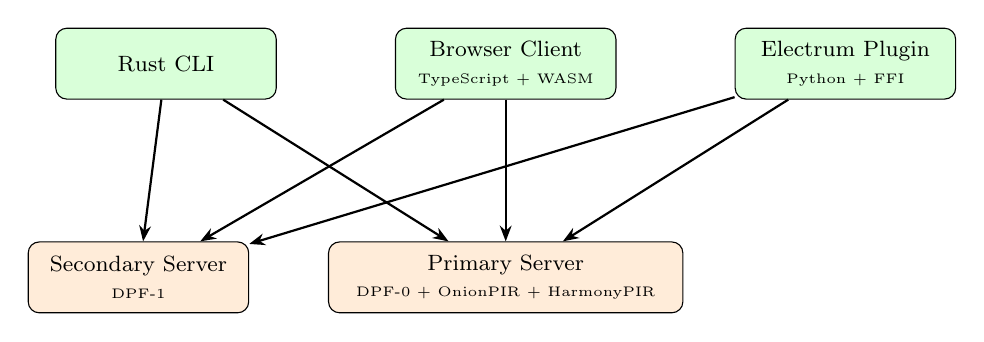
\begin{tikzpicture}[
    node distance=0.8cm and 1.2cm,
    box/.style={rectangle, draw, rounded corners, minimum width=2.8cm, minimum height=0.9cm, align=center, font=\footnotesize},
    arrow/.style={-{Stealth[length=2mm]}, thick},
    label/.style={font=\scriptsize, text=gray!70!black}
]

\node[box, fill=green!15] (webclient) {Browser Client\\{\tiny TypeScript + WASM}};
\node[box, fill=green!15, right=1.5cm of webclient] (electrum) {Electrum Plugin\\{\tiny Python + FFI}};
\node[box, fill=green!15, left=1.5cm of webclient] (cli) {Rust CLI};

\node[box, fill=orange!15, below=1.8cm of webclient, minimum width=4.5cm] (primary)
  {Primary Server\\{\tiny DPF-0 + OnionPIR + HarmonyPIR}};
\node[box, fill=orange!15, left=1cm of primary] (secondary) {Secondary Server\\{\tiny DPF-1}};

\draw[arrow] (cli) -- (primary);
\draw[arrow] (cli) -- (secondary);
\draw[arrow] (webclient) -- (primary);
\draw[arrow] (webclient) -- (secondary);
\draw[arrow] (electrum) -- (primary);
\draw[arrow] (electrum) -- (secondary);

\end{tikzpicture}
\caption{System architecture. A single \texttt{unified\_server} binary serves all three protocols, deployed as two instances: the primary hosts DPF server~0, OnionPIR, and both HarmonyPIR hint and query roles; the secondary hosts DPF server~1. A client connects to both instances for DPF-PIR, to the primary only for OnionPIR, and to either instance for HarmonyPIR (any two non-colluding nodes work).}
\label{fig:deployment}
\end{figure}

\textbf{Unified wire protocol.} All communication uses WebSocket with a compact binary protocol of the form \texttt{[4B length][1B request type][payload]}. The type code dispatches to one of the protocol handlers: generic requests (\texttt{0x01} \texttt{GET\_INFO}, \texttt{0x02} \texttt{GET\_DB\_CATALOG}, \texttt{0x04} \texttt{RESIDENCY}), DPF batch queries (\texttt{0x11} INDEX, \texttt{0x21} CHUNK), per-group Merkle verification (\texttt{0x33} sibling batch, \texttt{0x34} tree-top cache), HarmonyPIR (\texttt{0x40}--\texttt{0x43}: info, hints, single query, batch query), and OnionPIR (\texttt{0x51}--\texttt{0x56} for index/chunk queries and their Merkle variants). Legacy global-Merkle codes \texttt{0x31}/\texttt{0x32} are reserved for the earlier whole-table Merkle scheme and are not used by the current per-group implementation. The trailing byte on DPF batch queries optionally carries a database identifier for multi-database routing (Section~\ref{sec:deployment-catalog}).

\textbf{Unified server binary.} A single Rust binary, \texttt{unified\_server}, implements all three protocols and selects a role at startup:
\begin{itemize}[nolistsep,leftmargin=*]
    \item \textbf{Primary role:} Serves DPF batch queries (one of the two DPF shares), OnionPIR queries, and both HarmonyPIR hint streaming and HarmonyPIR online queries. Loads every database declared in its configuration file, the shared OnionPIR NTT store, and the per-group Merkle sibling tables. All databases and NTT data are memory-mapped via \texttt{memmap2}, so server startup is fast even for multi-gigabyte datasets. OnionPIR evaluation uses the SEAL library~\cite{seal} via Rust FFI. HarmonyPIR hint generation uses \texttt{rayon} for batch parallelism with the selected PRP backend (Hoang, FastPRP, or ALF).
    \item \textbf{Secondary role:} Serves the other DPF share only. A client connects to one primary and one secondary for the 2-server DPF-PIR protocol, ensuring that the two servers do not need to trust each other.
\end{itemize}
A production deployment typically runs one primary and one secondary on separate hosts, both exposing WebSocket endpoints. Because HarmonyPIR's hint and query roles can be split across any two non-colluding nodes, a client is free to pick any available primary as its HarmonyPIR query server and another as the hint server. For OnionPIR, the single server can be either instance, since OnionPIR does not rely on non-collusion.

\subsection{Browser Deployment via WebAssembly}

The browser client supports all three protocols through WebAssembly \cite{wasm} modules compiled from Rust:

\textbf{HarmonyPIR WASM.} Three independent WASM builds provide the PRP backends:
\begin{itemize}[nolistsep,leftmargin=*]
    \item \texttt{harmonypir/}: Hoang (swap-or-not) backend---smallest binary, no SIMD requirement.
    \item \texttt{harmonypir-fastprp/}: FastPRP backend---precomputed permutation tables.
    \item \texttt{harmonypir-alf/}: ALF backend with WASM SIMD128---fastest in browsers with SIMD support ($4$--$8\times$ over Hoang).
\end{itemize}

Each WASM module exports a \texttt{HarmonyGroup} class (whose original name in the codebase, \texttt{HarmonyBucket}, predates the bucket-to-group rename) with methods for hint loading, request building, response processing, and state serialization.

\textbf{OnionPIR WASM.} A $\sim$516~KB WASM module provides FHE key generation, query encryption, and response decryption. The client's secret key can be exported and reused across different OnionPIR instances with different database sizes, avoiding redundant key generation.

\textbf{Web Workers.} For HarmonyPIR, the client distributes the 155 group instances across 4 Web Workers, each running its own WASM instance. This parallelizes the request-building and response-processing phases, providing up to $4\times$ speedup on multi-core devices. Workers communicate via \texttt{Transferable} \texttt{ArrayBuffer}s to avoid serialization overhead.

\textbf{DPF-PIR in the browser.} DPF key generation and cuckoo hashing are implemented in pure TypeScript without WASM, as the operations (AES-based PRG expansion and XOR accumulation) are lightweight enough for JavaScript.

\subsection{Electrum Wallet Integration}

We provide a plugin for the Electrum Bitcoin wallet \cite{electrum} that replaces its native synchronization mechanism with PIR-based UTXO discovery.

\textbf{Plugin architecture.} The plugin hooks into Electrum's wallet lifecycle:
\begin{enumerate}[nolistsep,leftmargin=*]
    \item On wallet open, the plugin creates a \texttt{PirSynchronizer} that replaces Electrum's default \texttt{Synchronizer} (which sends script hashes to an Electrum server in the clear).
    \item The synchronizer collects all wallet addresses, converts them to RIPEMD-160 script hashes, and performs batch PIR queries to discover UTXOs.
    \item Discovered UTXOs are written back to the wallet's internal state, enabling normal spending operations.
\end{enumerate}

\textbf{Protocol selection.} Users choose between the three PIR backends via a Qt settings dialog:
\begin{itemize}[nolistsep,leftmargin=*]
    \item ``DPF 2-Server'': Pure Python DPF implementation with WebSocket transport.
    \item ``HarmonyPIR 2-Server'': Uses PyO3 FFI bindings to call the Rust HarmonyPIR library natively, providing near-Rust performance for PRP evaluation and state management.
    \item ``OnionPIRv2 1-Server'': Uses \texttt{ctypes} FFI to a pre-built native library (\texttt{libonionpir}) for FHE operations.
\end{itemize}

\textbf{Shared utilities.} All three backends share Python implementations of cuckoo hashing, PBC group derivation, VarInt decoding, and UTXO data parsing---mirroring the Rust and TypeScript implementations to ensure cross-platform consistency.

\subsection{Database Catalog and Client Sync}
\label{sec:deployment-catalog}

A single unified server can host multiple logically distinct databases at once. The canonical deployment combines one \emph{full} checkpoint (a complete UTXO snapshot at some block height) with a family of \emph{delta} databases that encode the diffs between successive checkpoints (Section~\ref{sec:delta-db}). The server loads all databases at startup from a \texttt{databases.toml} configuration file that declares, for each entry, a name, type (\texttt{full} or \texttt{delta}), base and tip block heights, on-disk path, and a warmup priority.

\textbf{Wire-level routing.} Each loaded database is assigned a small integer \texttt{db\_id}, with the main checkpoint at \texttt{db\_id=0}. To query a specific database, the client appends a one-byte \texttt{db\_id} to its \texttt{INDEX\_BATCH}/\texttt{CHUNK\_BATCH} request. Requests without the trailing byte are routed to \texttt{db\_id=0}, preserving backward compatibility with single-database clients. The same routing is used for Merkle sibling and tree-top requests.

\textbf{Catalog endpoint.} A new request \texttt{GET\_DB\_CATALOG} (\texttt{0x02}) returns the full list of databases currently served. Each catalog entry contains the \texttt{db\_id}, type, base height, tip height, cuckoo parameters (index and chunk bin counts, tag seed), and a flag indicating whether per-group Merkle verification data is available for that database. The top-level \texttt{GET\_INFO} (\texttt{0x01}) response additionally embeds a \texttt{"databases"} array with per-database Merkle metadata (arity, level sizes, per-group roots, super-root, and tree-top hash), so that a client can verify Merkle proofs against the correct database without a second round trip.

\textbf{Client sync planning.} Given the catalog and the client's last synced height $h_\text{last}$, the client computes a \emph{sync plan}: an ordered sequence of database queries that advances from $h_\text{last}$ to the latest available tip. The plan is chosen by the following rule:
\begin{enumerate}[nolistsep,leftmargin=*]
    \item If $h_\text{last}$ is absent or $0$, pick the highest-tip full checkpoint as a single-step fresh sync.
    \item If $h_\text{last}$ already equals the latest tip, the plan is empty.
    \item Otherwise, search for a chain of deltas whose base/tip heights connect $h_\text{last}$ to the tip. The search is breadth-first over the delta graph, capped at a configurable maximum chain length (currently 5).
    \item If no suitable chain exists, or it exceeds the cap, fall back to the latest full checkpoint.
\end{enumerate}
The sync plan is a pure function of the catalog and $h_\text{last}$: it performs no I/O and can be computed entirely on the client. The client then executes each step by replaying its standard DPF/HarmonyPIR/OnionPIR query pipeline against the appropriate \texttt{db\_id}.

\subsection{Practical Considerations}

\textbf{Server deployment.} Production servers are deployed behind reverse proxies (e.g., nginx) with TLS termination via Cloudflare Tunnel, providing WSS (WebSocket Secure) transport without exposing server IP addresses.

\textbf{Database updates.} When the Bitcoin UTXO set changes (approximately every 10 minutes with each new block), the server operator re-runs the database generation pipeline for the relevant checkpoint and, optionally, publishes a new delta keyed to the previous checkpoint. For DPF-PIR and HarmonyPIR, an update only affects the cuckoo hash tables and sibling/tree-top files. For OnionPIR, the NTT preprocessing must also be recomputed, which takes approximately 95 seconds. The \texttt{databases.toml} file is updated to declare the new database, and clients discover it at their next \texttt{GET\_DB\_CATALOG} call.

\textbf{Dust filtering.} UTXOs of $576$ satoshis or less, and addresses with more than $100$ UTXOs, are filtered during database generation. This removes dust outputs and whale addresses (who should run full nodes), reducing the database size and improving PIR efficiency for typical light-client queries. See Section~\ref{sec:extension} for the rationale.


\clearpage

\section*{Acknowledgments}

We thank \href{https://wuwuz.github.io/}{Mingxun Zhou} for advice and suggestions on stateful PIR and their implementations. We thank \href{https://sites.google.com/view/renling}{Ling Ren} and \href{https://scholar.google.com/citations?user=f54M0ikAAAAJ&hl=en}{Pranav Shriram Arunachalaramanan} for advice and suggestions on state-of-the-art PIR schemes in various settings, batch PIR, and understanding of the SimplePIR family of protocols.

\bibliography{refs}

\end{document}
